 \begin{figure}[h]
  \centering
  \includegraphics[scale = .5]{fig/dbn.png}\\
  \caption{Deep learning procedure}
\end{figure}
In 2006, a new feature learning and deep learning method was initiated by G.Hinton and has brought great impact in both academic and industrial field. This deep learning method is a kind of deep neural network which contains several layers. The core idea, referred to as \emph{greedy layerwise unsupervised pretraining} was to learn the bottom to top hierarchical features in a deep neural network. In deep learning, each layer is trained separately which makes is really fast and the output of the lower layer is the input of the higher one. When using greedy layerwise unsupervised pretraining, the two conjunctival layers can regarded as a Restrict Boltzman Machine (RBM) and the \emph{Energy} of the RBM is defined as\cite{Hinton12}:
\begin{equation}\label{eq:engery}
  E(v,h) =  - \sum\limits_{i \in visible} {{a_i}{v_i}}  - \sum\limits_{j \in hidden} {{b_j}{h_j}}  - \sum\limits_{i,j} {{v_i}{h_i}{w_{ij}}}
\end{equation}
Here, $v_i$, $h_j$ are the visible value (input) and the hidden value (output) respectively, and $a_i$, $b_j$ are their bias . $w_{ij}$ is the weight of the visible node $i$ and hidden node $j$. The probability that the RBM can recall the visible vector, $v$, is defined as:
\begin{equation}
\begin{gathered}
  p(v) = \frac{1}{Z}\sum\limits_h {{e^{ - E(v,h)}}} \\
   Z = \sum\limits_{i,h} {{e^{ - E(v,h)}}}  \\
\end{gathered}
\end{equation}
The derivative of the log probability of a training vector with respect to a weight is:
\begin{equation}
\begin{gathered}
  \frac{{\delta \log p(v)}}{{\delta {w_{ij}}}} = {\left\langle {{v_i}{h_j}} \right\rangle _{data}} - {\left\langle {{v_i}{h_j}} \right\rangle _{model}}\\
  {\left\langle {{v_i}{h_j}} \right\rangle _{model}} \approx {\left\langle {{v_i}{h_j}} \right\rangle _{recon}}\\
  \end{gathered}
\end{equation}\label{eq:weight}

\begin{figure}[h]
\centering
\def\layersep{1.5cm} % Gap between visible & hidden units
\def\numvis{3} % Number if visible units
\def\numhid{4} % Number of hidden units
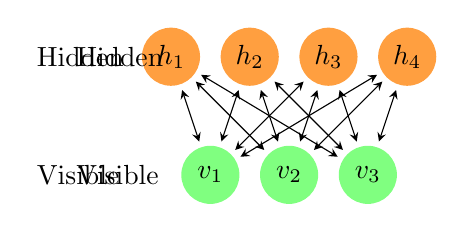
\begin{tikzpicture}[
    node distance=\layersep,
    line/.style={<->,shorten >=2pt,shorten <=2pt,>=stealth}
    ]
    \tikzstyle{neuron}=[circle,fill=black!25,minimum size=21pt,inner sep=0pt];
    \tikzstyle{visible neuron}=[neuron, fill=green!50];
    \tikzstyle{hidden neuron}=[neuron, fill=orange!75];
    \tikzstyle{annot}=[text width=4em];

    % Iterate over visible units
    \foreach \name / \y in {1,...,\numvis}
        \node[visible neuron] (V\name) at (\y,0) {$v_\y$};

    % Iterate over hidden units
    \foreach \name / \y in {1,...,\numhid}
        % Calculate the appropriate offset for the hidden unit based on the
        % number of visible units.
        \pgfmathparse{\y + (\numvis - \numhid) * 0.5}
        \node[hidden neuron] (H\name) at (\pgfmathresult, \layersep) {$h_\y$};

    % Draw a double-arrow connector between the each unit
    \foreach \source in {1,...,\numvis}
        \foreach \dest in {1,...,\numhid}
            \draw[line] (V\source) -- (H\dest);

    % use if/then/else to decide where to draw the labels
    \ifthenelse{\numvis > \numhid}
    {
        \node[annot,left of=V1, node distance=1cm] (hl) {Visible};
        \node[annot,above of=hl] {Hidden};
    }
    {
        \node[annot,left of=H1, node distance=1cm] (hl) {Hidden};
        \node[annot,below of=hl] {Visible};
    }
\end{tikzpicture}
\label{fig:rbmtopology}
\caption[RBM Topology]{Restricted Boltzmann topology with \numvis{} visible units and \numhid{} hidden units.}
\end{figure}

Even though,  the ${\left\langle {{v_i}{h_j}} \right\rangle _{model}}$ can't be calculated, Hinton proposed a fast learning procedure, called \emph{Contrastive Divergence}, that can estimate it by ignoring the tricky term in the objective function and proved that this can lead to the convergence. Sutskever and Tieleman have shown that this procedure is not following the gradient of any function\cite{SutskeverT10}.
\begin{figure}
  \centering
  % Requires \usepackage{graphicx}
  \includegraphics[scale=.5]{fig/deeplearning.pdf}\\
  \caption{Hierarchical Representation of Deep Learning}
\end{figure}

After this greedy layerwised unsupervised pretraining, the configuration of the deep network can be the initial of the supervised deep neural network predictor\cite{Srivastava13}. And the stochastic gradient descent can be applied for further optimization. The initial configuration after greedy layerwised unsupervised pretraining can make this deep network get rid of the local minimum since the supervised procedure is not based on any gradient method.

It is interesting to ask why this greedy layerwise unsupervised pretraining can help in supervised learning\cite{ErhanCBV10}. The curriculum greedy layerwise unsupervised pretraining tries to build some intermediate representations rather than some distinguishable representations. This is nicely related to curriculum learning idea which indicates that it is much more easier to learn some simpler concept first and build a much more complicated ones on top of the simpler ones\cite{BengioICML09}. For a deep supervised classifier, in the unsupervised training procedure, the deep neural network is the stacked RBMs which can initialize in a \emph{good} local minimum where the \emph{good} refers to low generalization error\cite{Bengio13}.

Stacked RBMs has been developed for many large learning problems as the feature extractor for other supervised classifiers. In these cases, stacked RBM is used as both feature extractor to learn the hierarchical representations and autoencoder to evaluate the similarity between the features and the images.  However, single-layer RBM can still be a good predictor for a supervised learning problems. H.Larochelle used the RBM stand-alone to build the discriminative RBM on character recognition without replying on any other classifier\cite{LarochelleB08}. Even though, for the large learning task, deep neural network with millions or even billions of nodes can get some good results\cite{krizhevsky2012imagenet}\cite{LeRMDCCDN12}, in some simple shadow network can still do well. It's a big waste to use a cannon to kill a mosquito.

When training the deep neural network, there are many details that can speed the convergency of the stacked RBMs to achieve a better local minimum. Cho et al. proposed a adaptive learning rate for the RBM training as well as a novel gradient estimator that takes into account the invariance of the model to flipping hidden unit bits and inverting signs of corresponding weight vectors\cite{cho2011}.  For the choice of the hidden units, several experiments have shown that nonlinearity could influence both training and generalization performance\cite{GlorotB10}\cite{GlorotBB11}\cite{NairH10}. Moreover, the initial weights can affect the training results. A good initialization can substantially reduce the difficulty of training the deep neural network. With a sparse initialization or using often saturated nonlinearities, it is more promising to make the hidden units specialized\cite{martens2010deep}. For the training method, there is still a debate between online learning method such as stochastic gradient descent and using large mini batch(thousands of samples)\cite{LeNCLPN11},  even though, the stochastic gradient descent and its invariants are more popular and have won many competitions. As we can see in Equation (\ref{eq:weight}), most of the computation in updating the weights can be done with matrix operations, it is more convenient to use GPU to do these jobs which is designed to accelerate the matrix operations\cite{raina2009large}. Normally, training the huge deep network on GPU can be at least 10 times faster than training on CPU.

Despite great achievement in both academic and industrial area, there are still some criticisms, one of which is that there are so many hyperparameters and variants that exploring the configuration and the architecture is really an art\cite{LeCunBOM12}. To solve this problem, many automating hyperparameters searching works have been proposed recently which makes it more convenient and efficient\cite{BergstraB12}\cite{BergstraBBK11}\cite{snoek2012practical}. To deal with large quantities of image recognition problem, deep learning can be the first choice. As a neural network, it can easily get rid of the local  minimum, which is the biggest issue in all the large neural network training procedure, with just a little prior knowledge through the efficient unsupervised training. However, recent work on large quantities of labeled data shows that with a proper initialization, the pure deep supervised network can still be successfully trained without any layerwised pre-training\cite{cirecsan2010deep}\cite{glorot2011deep}\cite{seide2011conversational}. And in this situation, the layerwised unsupervised pretraining can bring little or even no improvement over the supervised one when training for long enough.

In addition, deep learning will be the most promising method for image recognition in the next few years. Even though pure supervised learning can compete with deep learning while there are enough labeled data for training, still deep learning and unsupervised pre-training for image recognition would be the future. As in real world, we can always obtain enough data while just a very small fraction can be labeled. Unsupervised feature extraction techniques can be a more realistic method. 

